\documentclass{article}
\usepackage{amsthm,amsfonts}
\usepackage{graphicx}

% 
%\usepackage{amsthm}

\newcommand{\centeripe}[1]{\begin{center}\Ipe{#1}\end{center}}
\newcommand{\comment}[1]{}

\newcommand{\centerpsfig}[1]{\centerline{\psfig{#1}}}

\newcommand{\seclabel}[1]{\label{sec:#1}}
\newcommand{\Secref}[1]{Section~\ref{sec:#1}}
\newcommand{\secref}[1]{\mbox{Section~\ref{sec:#1}}}

\newcommand{\alglabel}[1]{\label{alg:#1}}
\newcommand{\Algref}[1]{Algorithm~\ref{alg:#1}}
\newcommand{\algref}[1]{\mbox{Algorithm~\ref{alg:#1}}}

\newcommand{\applabel}[1]{\label{app:#1}}
\newcommand{\Appref}[1]{Appendix~\ref{app:#1}}
\newcommand{\appref}[1]{\mbox{Appendix~\ref{app:#1}}}

\newcommand{\tablabel}[1]{\label{tab:#1}}
\newcommand{\Tabref}[1]{Table~\ref{tab:#1}}
\newcommand{\tabref}[1]{Table~\ref{tab:#1}}

\newcommand{\figlabel}[1]{\label{fig:#1}}
\newcommand{\Figref}[1]{Figure~\ref{fig:#1}}
\newcommand{\figref}[1]{\mbox{Figure~\ref{fig:#1}}}

\newcommand{\eqlabel}[1]{\label{eq:#1}}
\newcommand{\eqref}[1]{(\ref{eq:#1})}

\newtheorem{thm}{Theorem}{\bfseries}{\itshape}
\newcommand{\thmlabel}[1]{\label{thm:#1}}
\newcommand{\thmref}[1]{Theorem~\ref{thm:#1}}

\newtheorem{lem}{Lemma}{\bfseries}{\itshape}
\newcommand{\lemlabel}[1]{\label{lem:#1}}
\newcommand{\lemref}[1]{Lemma~\ref{lem:#1}}

\newtheorem{cor}{Corollary}{\bfseries}{\itshape}
\newcommand{\corlabel}[1]{\label{cor:#1}}
\newcommand{\corref}[1]{Corollary~\ref{cor:#1}}

\newtheorem{obs}{Observation}{\bfseries}{\itshape}
\newcommand{\obslabel}[1]{\label{obs:#1}}
\newcommand{\obsref}[1]{Observation~\ref{obs:#1}}

\newtheorem{assumption}{Assumption}{\bfseries}{\rm}
\newenvironment{ass}{\begin{assumption}\rm}{\end{assumption}}
\newcommand{\asslabel}[1]{\label{ass:#1}}
\newcommand{\assref}[1]{Assumption~\ref{ass:#1}}

\newcommand{\proclabel}[1]{\label{alg:#1}}
\newcommand{\procref}[1]{Procedure~\ref{alg:#1}}

\newtheorem{rem}{Remark}
\newtheorem{op}{Open Problem}

\newcommand{\etal}{\emph{et al}}

\newcommand{\voronoi}{Vorono\u\i}
\newcommand{\ceil}[1]{\left\lceil #1 \right\rceil}
\newcommand{\floor}[1]{\left\lfloor #1 \right\rfloor}


\newtheorem{lem}{Lemma}
\newtheorem{thm}{Theorem}
\newtheorem{clm}{Claim}
\newtheorem{prop}{Proposition}
\newcommand{\cn}{\mathsf{cr}}
\newcommand{\dn}{\mathsf{dn}}
\newcommand{\wdn}{\mathsf{wdn}}
\newcommand{\killtext}[1]{}


\begin{document}

\begin{thm}[Klaus' Warm-Up Exercise I]\label{thm:klaus1}
Let $s(k)$ and $d(k)$ be such that $s(k)\times d(k)=O(k^{1-\epsilon})$
for some positive constant $\epsilon > 0$ and let $1<c\le 2$ be some
constant.  Then there exists a value
$k_0$ such that for all $k\ge k_0$, it is not possible to draw any
binary tree of height $k$ with at least $c^k$ leaves
using $d(k)$ distinct edge lengths and
$s(k)$ distinct slopes.
\end{thm}

\begin{proof}
Consider a complete binary tree $T$ of height $k$ and suppose it is
drawn using $s(k)$ slopes and $d(k)$ edge lengths.  Then any root to
leaf path in $T$ consists of a sequence of vectors of which there are
at most $\ell=2s(k)\times d(k)=O(k^{1-\epsilon})$ types.  Furthermore,
the final location of a leaf depends only on the number of each type
of vector used and not on the order in which they appear.  Thus, there
are only 
\[
           {k+\ell-1 \choose \ell} \le k^\ell = k^{O(k^{1-\epsilon})}
\]
possible locations for the leaves of $T$.  However, $T$
has at least $c^k$ leaves.  Thus, for any $k$ such that $c^k> k^\ell$ there
must be at least two leaves of $T$ at the same location.
\end{proof}

\begin{thm}[Klaus' Warm-Up Exercise II]\label{thm:klaus2}
Let $0<\alpha<\pi$ be any constant and let $d(k)=O(k^{1/2-\epsilon})$
for some constant $\epsilon > 0$.  Then there exists some 
value $k_0$ such that for all $k> 0$ it is not possible to draw a
complete binary tree of height $k$ using at most $d(k)$ edge lengths
and for which, for each node $v$ with parent $u$ and child $w$ $\angle
uvw\in\{-\alpha,\alpha\}$.
\end{thm}

\newcommand{\rwlen}{ck^{1/2}}

\begin{proof}
By the theory of random walks, there exists a set of $r=\Omega(2^{k})$
leaves in $T$ such that the path from the root to each of these leaves
never has a number of right turns exceeding the number of left turns,
or vice versa, by more than $\rwlen$ \cite{X}.  Thus, along all these
$r$ paths the number of slopes of edges is bounded by $2\rwlen$.  The
result now follows from Theorem~\ref{thm:klaus1}.
\end{proof}


\begin{lem}\label{lem:random-walk}
Let $T$ be a complete rooted binary tree of depth $k$ and let each
edge of $T$ be labelled with a vector of length $t$ having exactly
$t-1$ zero entries and exactly $1$ entry in $\{+1,-1\}$.  Furtermore,
for each internal node $v$ of $T$, the two edges from $v$ to its
children have different labels.

Call the \emph{value} of a vertex $v$ the sum of all vectors on the
path from the root of $T$ to $v$.  Then there exists a set of
$\Omega(c_t^k)$ root to leaf paths in $T$ such that the vertices on
these paths have only $O(k^{1-\epsilon_t})$ different values, where
$c_t > 1$ and $\epsilon_t > 0$ depend only on $t$.
\end{lem}

\begin{proof}
Too hard.
\end{proof}

\begin{thm}
There exists outerplanar graphs $G$ with $\wdn(G) > 2$.
\end{thm}

\begin{proof}
Let $G$ be the ``complete'' outerplanar graph of depth $k$.  Suppose
that $G$ is drawn using 2 edge lengths, say $a$ and $b$.  Then the
triangles of $G$ come in 4 types: (1)~isoscelese triangles with 2
sides of length $a$ and one side of length $b$, (2)~isoscelese
triangles with 2 sides of length $b$ and one side of length $a$,
(3)~equilateral triangles of side length $a$ and (4)~equilateral
triangles of side length $b$.  For each type of triangle, draw the
circumcircle about select a
point in its interior and call that point the \emph{center} of the
triangle.

Consider the point $p$ that is the center of the root triangle of $G$.
For any other center $q$ there is a unique path from $p$ to $q$ that
consists of a sequence of centers where each consecutive pair of
centers come from two triangles that share an edge.  This path can be
viewed as a sequence of at most $k$ vectors.  These vectors have at
most $4^2=16$ different lengths.  Furthermore, two consecutive vectors
differ in direction by one of at most 16 (32?) different angles.  Call
these angles $\alpha_1,\ldots,\alpha_{16}$.  Thus, the direction of
any particular vector can be written as $\sum_{i=1}^{16} k_i\alpha_i$
where each $k_i$ is an integer.  By Lemma~\ref{lem:random-walk}, there
exists a set of $\Omega(c_{16}^k)$ centers, each of which is the sum
of $k$ vectors, at most $\ell=O(k^{1-\epsilon_{16}})$ of which are
distinct.  Therefore, there are at most
\[
     {k+\ell-1 \choose \ell} \le k^{O(k^{1-\epsilon_{16}})}    
\]
Therefore there must be at least
$\Omega(c_{16}^k)/k^{O(k^{1-\epsilon_{16}})}$ centers that are at the
same location.  As there are only 4 different types of triangles and
$k^{O(k^{1-\epsilon_{16}})}$ different orientations of the triangles we
conclude that, for sufficiently large $k$, there must be at least 2
triangles of the same type and orientation.  Thus, the three vertices
of these two triangles of $G$ are assigned the same locations.
\end{proof}

\killtext{
\begin{thm}
There exist outerplanar graphs $G$
\end{thm}

\begin{thm}
For any outerplanar graph $G$, $\dn(G)\le 3$.
\end{thm}

\begin{proof} 
Without loss of generality, we may assume that $G$ is maximal
outerplanar.  A \emph{triangle} of $G$ is a cycle of length 3.  A
drawing of $G$ using only three edge lengths is obtained as follows:
Consider the \emph{dual graph} $T$ of $G$ whose vertices are the
triangles of $G$ and in which two triangles are adjacent if and only
if they share an edge.  It is well-known that, since $G$ is maximal
outerplanar, $T$ is a binary tree. Select an arbitrary triangle of $G$
to act as the root of $T$ and call this triangle the \emph{root
triangle}.

We locate the root triangle's vertices at the points $p=(0,0)$,
$q=(1,0)$ and some point $r=(x,y)$ in the unit square $[0,1]^2$ whose
coordinates will be specified later.  Consider any triangle $uvw$ of
$G$ that is not the root triangle and assume (recursively) that the
three vertices of the parent $uvw'$ of $uvw$ have already been
assigned locations.  The location of $w$ is then obtained by
reflecting $w'$ through the line containing $u$ and $v$.  In this way,
each vertex of $G$ is assigned a location that is determined entirely
by the choice of $r$.

We will show that there is a choice of the point $r$ that results in
a drawing of $G$ by showing that, for any vertex-edge pair
$(v,e)$, the set of choices of $r$ for which $v$ is located in
$e$ is a 1-dimensional set.\footnote{A set $S$ of points in the
plane is a 2-dimensional set if it contains a disk of positive radius.
If $S$ is not 2-dimensional but contains a finite curve then $S$ is
1-dimensional.  If $S$ is non-empty but is neither 1-dimensional nor
2-dimensional then $S$ is $0$-dimensional.} Thus, the set of choices
of $r$ for which some vertex lies on some edge is a finite union of
1-dimensional sets, and is therefore also 1-dimensional.  However,
$r$ can be selected to be any point in $[0,1]^2$, a 2-dimensional
set, so it suffices to select any $r$ that is not in this
1-dimensional set.

We require the following geometric result:

\begin{clm}
Let $f_v:[0,1]^2\mapsto\mathbb{R}^2$ be the function that determines
the location of vertex $v$ given the location of $r$.  For any vertex
$v$ not adjacent to $p$ nor $q$ the range of $f_v$ is 2-dimensional
\end{clm}


Note that, since the root triangle is selected arbitrarily, we may
assume that $e$ is an edge of the root triangle.  We distinguish
between two cases.  In the first case, $e$ is the segment $pq$, i.e.,
the bottom edge of the root triangle.  Let $f:[0,1]^2\mapsto
\mathbb{R}^2$ be the function that defines the location of $v$ given
the location of $r$.  The codomain (range) of $f$ is 2-dimensional and
the intersection of the segment $pq$ with this set is 1-dimensional.
The preimage of $pq$ in $f$ is a 1-dimensional subset of $[0,1]^2$, as
required.

Next we consider the case where $e$ is one of the other two edges of
the root triangle, say the segment $pr$.  In this case, consider the
representation of $r$ using polar coordinates $(\ell,\theta)$ where
$\ell=\|pr\|$ and $\theta=\angle qpr$.  By a change of coordinates, we
may assume that the segment $pr$ is contained in the $x$-axis so that
the root triangle has vertices $p=(0,0)$, $r=(-\ell,0)$ and
$q=(-\cos\theta,\sin\theta)$.  Again, the parameters $\ell$ and
$\theta$ can be selected from a 2-dimensional set and there is a
function $g$ that defines the location of $v$ given $\ell$ and
$\theta$ and the codomain of $g$ is 2-dimensional.  Note that, if
$g(\ell,\theta)$ is contained in the segment $pr$ then
$g(\ell,\theta)$ is on the $x$ axis.  The preimage of the $x$-axis in
$g$ is a 1-dimensional subset of the 2-dimensional set that describes
all valid choices of $\ell$ and $\theta$ and this corresponds to a
1-dimensional subset of $[0,1]^2$ which describes all valid choices of
$x$ and $y$, as required.  
\end{proof}

Note that, without some further ideas, it is not possible to
generalize the above proof to show that $\dn(G)\le 2$ if $G$ is
outerplanar.  In particular, with only two distance classes, all
triangles of $G$ are isosceles triangles defined by a single parameter
$\alpha$ that measures the angle at the apex.  In this case, the range
of the function $g$ is a 1-dimensional set and this set can coincide
with the line containing $pr$.  The example in the figure below
shows an example where this occurs.  In this example, any choice
of $\alpha$ in the interval $[0,\pi/6]$ results in the vertex $v$ being
embedded on the segment $pr$.

\begin{tabular}{cccc}
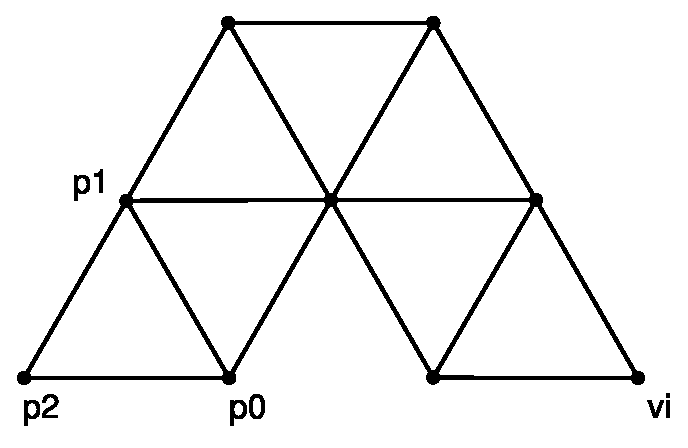
\includegraphics[scale=.30]{no2-1} &
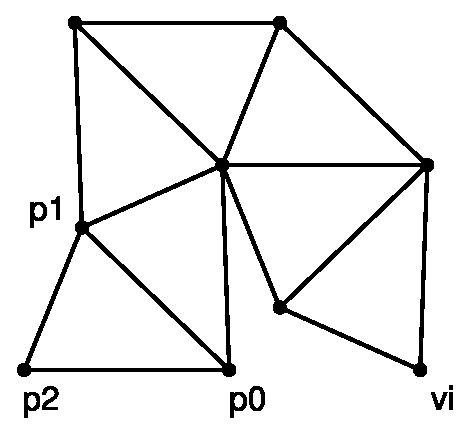
\includegraphics[scale=.30]{no2-2} &
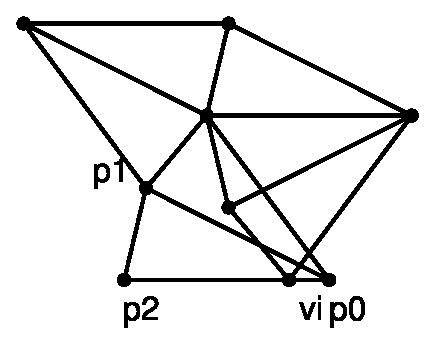
\includegraphics[scale=.30]{no2-3} &
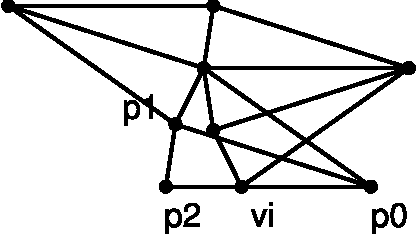
\includegraphics[scale=.30]{no2-4} 
\end{tabular}

It is easy to observe that there are outerplanar graphs with distance
number greater than 1.  Consider for example the graph comprised of
one degree-6 vertex adjacent to each vertex of a path of length 6. 
}

For edge-maximal outerplanar graphs, in fact for all weak planar
triangulations,\footnote{A planar graph is a \emph{weak triangulation}
if it has an embedding where the edges on the unbounded face form a
cycle and the edges of the bounded faces form 3-cycles.} we can decide
whether they have distance number 1.

\begin{prop} 
A weak planar triangulation $G$ has distance number 1 if and only if
it is a subgraph of the triangular grid.\footnote{The triangular grid
is the infinite graph with vertex set $V=\{(i+j/2,j\sqrt{3}/2):
i,j\in\mathbb{Z}\}$ and in which two vertices are adjacent if and only
if the Euclidean distance between them is 1.\label{fna}}  Furthermore,
testing if an $n$-vertex weak planar triangulation has distance number
1 can be done in $O(n)$ time.  
\end{prop}

\begin{proof}
The characterization part of the proposition follows immediately from
the fact that the assignment of vertex locations to the vertices of
$G$ is unique, up to the choice of location of one triangle of $G$.

To obtain an efficient algorithm for testing if $G$ is a subgraph of
the triangular grid  we can compute any spanning tree $T$ of the dual
graph of $G$. By assigning the root of $T$ to be a grid triangle
adjacent to the origin and traversing $T$ we can, in linear time,
obtain locations for all vertices of $G$.  This provides vertex
locations for $G$ such that each vertex is located on a point of the
triangular grid.  All that remains to check is that each edge has unit
length and that no two vertices are assigned to the same grid point.

Checking that each edge of $G$ has unit length is trivially done in
constant time per edge.  To check that no two vertices of $G$ are
assigned to the same grid point we observe that the points of the
triangular grid can be uniquely indexed by pairs of integers (see
Footnote~\ref{fna}).  Furthermore, for the vertex locations of $G$ these
integers are in the set $\{-n,\ldots,n\}$.  Thus, using radix sort we
can, in $O(n)$ time, sort the vertices of $G$ by their location to
determine if any two vertices are assigned the same location.
\end{proof}

\end{document}
